\documentclass[fleqn]{article}
\usepackage[utf8]{inputenc}
\usepackage{amsmath}
\usepackage{lmodern} % for bold teletype font
\usepackage{listings}
\usepackage[export]{adjustbox}
\usepackage{subcaption}
\usepackage{graphicx}
\usepackage{xcolor}   % for \textcolor
\usepackage{float}
\usepackage{array}
\usepackage{tabu}

\lstset{
  basicstyle=\ttfamily,
  columns=fullflexible,
  frame=single,
  breaklines=true,
  postbreak=\mbox{\textcolor{red}{$\hookrightarrow$}\space},
}

\title{Static Resource Allocation}
\author{Mark Towers}
\date{June 2019}

\begin{document}
\maketitle

\section{Problem Statement}\label{sec:problem-statement}
In prior research into resource pricing for resource allocation within cloud computing, job's considered have had fixed resource requirements that server's must fulfill.
However in this research we consider job's that have requirements that must be fulfill with a deadline so that the resource allocation must allow the deadline consider to be true.
We have then developed a greedy algorithm to solve the problem to maximise the social welfare where the total utility is known of each jobs.
However in real life then server's that run the job would want to be payed to run a job so we have developed new auction. \\
In the new section, we will describe the problem case and how we generated a model. \\

\section{Problem Case}\label{sec:problem-case}
\subsection{Variable}\label{subsec:variable}
There are J jobs, indexed with $ j = 1,\dots,J $ and I servers, indexed with $ i = 1,\dots,I $.
\begin{itemize}
    \item $ x_{i,j} \in \{0, 1\}$ indicates whether the job $j$ was done on server $i$
    \item $ s_{i,j} $ the rate that the program is loaded at (MB/s)
    \item $ w_{i,j} $ the rate of computation (TFlop/s)
    \item $ r_{i,j} $ the rate that the result's data is sent back (MB/s)
\end{itemize}

\subsection{Constants}\label{subsec:constants}
Server - i
\begin{itemize}
    \item Maximum storage - $ S_i $ (MB)
    \item Maximum computation capacity - $ W_i $ (TFlop/s)
    \item Maximum communication bandwidth - $ R_i $ (MB/s)
\end{itemize}
Job - j
\begin{itemize}
    \item Required storage - $ s_j $ (MB)
    \item Required computation capacity - $ w_j $ (TFlop)
    \item Required data for results - $ r_j $ (MB)
    \item Utility - $ U_j $ (\$)
    \item Deadline - $ D_j $ (s)
\end{itemize}

\subsection{Optimisation}\label{subsec:optimisation}
\begin{align}
    max \sum_{j=1}^{J} U_j x_{i,j} && \forall i = 1,\dots,I
\end{align}

\subsection{Constraints}\label{subsec:constraints}
Job to server allocation
\begin{align}
    \sum_{i=1}^I x_{i,j} \leq 1 && \forall j = 1,\dots,J \\
    x_{i,j} \in \{0, 1\} && \forall i = 1,\dots,I; j = 1,\dots,J
\end{align}

%% Server resources checking
Server resource available
\begin{align}
    \sum_{j=1}^J s_j x_{i,j} \leq S_i && \forall i = 1,\dots,I
\end{align}
\begin{align}
    \sum_{j=1}^J w_{i,j} x_{i,j} \leq W_i && \forall i = 1,\dots,I
\end{align}
\begin{align}
    \sum_{j=1}^J (r_{i,j} + s_{i,j}) x_{i,j} \leq R_i && \forall i = 1,\dots,I
\end{align}

%% Within deadline
Process completed within deadline
\begin{align}
    \frac{S_j}{s_{i,j}} + \frac{W_j}{w_{i,j}} + \frac{R_j}{r_{ij}} \leq D_j && \forall i = 1,\dots,I; j = 1,\dots,J
\end{align}

Resource usage
\begin{align}
    0 \le s_{i,j} && \forall i = 1,\dots,I; j = 1,\dots,J
\end{align}
\begin{align}
    0 \le w_{i,j} && \forall i = 1,\dots,I; j = 1,\dots,J
\end{align}
\begin{align}
    0 \le r_{i,j} && \forall i = 1,\dots,I; j = 1,\dots,J
\end{align}

\subsection{Problem Case Explanation}\label{subsec:problem-case-explanation}
\begin{itemize}
    \item Equation 1 is the objective function that maximises the sum of the job utility for jobs completed.
    \item Equation 2 and 3 enforce that a job is only done on a single server.
    \item Equations, 4 to 6, ensures that the server resource used are within the maximum resources available.
    \item Equation 7 enforces that the job will be completed within the deadline on only the servers that is a job runs on.
    \item Equations, 8 to 10, ensures that resource speeds are within a valid range of greater than 0
\end{itemize}

\subsection{Example cases}\label{subsec:example-cases}
\begin{figure}[H]
    \begin{subfigure}{0.5\textwidth}
        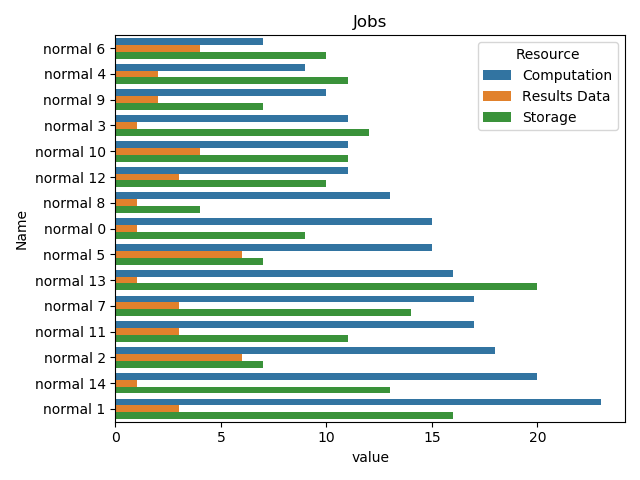
\includegraphics[width=1\linewidth, height=5cm]{/images/jobs.png}
        \caption{Example jobs}
    \end{subfigure}
    \begin{subfigure}{0.5\textwidth}
        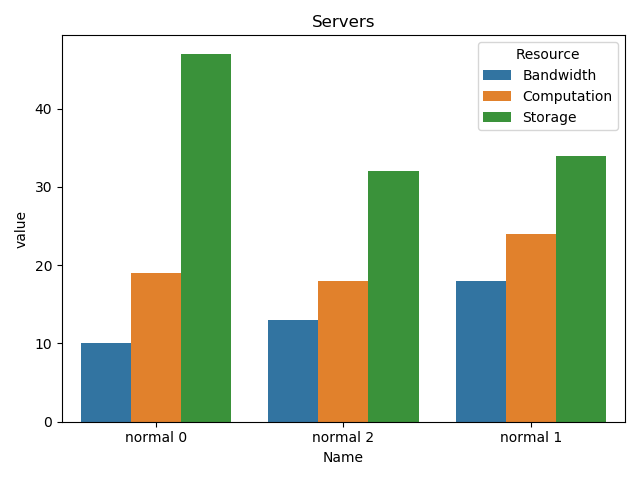
\includegraphics[width=1\linewidth, height=5cm]{/images/servers.png}
        \caption{Example Servers}
    \end{subfigure}

    \caption{Example jobs and servers}
\end{figure}

\subsection{Model creation}\label{subsec:model-creation}
To create each of the jobs and servers we choose a mean and standard deviation for each attribute that is then
used to generate a random number from a normal distribution.
We normalise the value generated to make it an integer and check that the value is greater than zero. \\

\begin{tabu} to 1\textwidth { | X[l] | X[l] | X[l] | X[l] | X[l] | X[l] | }
\hline
Job Attribute & Mean & Std & Server Attribute & Mean & Std \\
\hline
Storage & 10 & 4 & Storage & 45 & 10 \\
\hline
Compute & 15 & 5 & Compute & 30 & 5 \\
\hline
Results data & 5 & 4 & Bandwidth & 40 & 5 \\
\hline
Utility & 50 & 20 & & & \\
\hline
Deadline & 15 & 4 & & & \\
\hline
\end{tabu}

%% Todo Redo, Plot job and server


\section{Greedy Algorithm}\label{sec:greedy-algorithm}
The problem case laid out above is a knapsacking variation which has been shown to be NP-Hard to solve optimality.
Therefore while a solution can be found through integer programming, it is extremely slow to do and become impossible to solve for
problem cases with more than 15 jobs and 3 servers on a regular computers. \\
This means that to calculate the optimal solution, with full knowledge, then a greedy algorithm must be developed.
To do this, I have created two greedy algorithm that are compared and explained below. \\

\subsection{Greedy implementation}\label{subsec:greedy-implementation}
The first algorithm is a three stage process where the jobs are sorted on how good they are based on a metric like the
ratio of utility to resource's required. Then For each jobs in order of value, a server is selected for the jobs to run
on based on the another metric like which server has the least resources available. Resources are then allocated to a
job based on a third policy that calulcates the values for each possible allocation like the percentage of the available
resource that the allocated resources would use. The maximum of this is then chosen and allocated for the job on the server
with the process repeated till no jobs can be allocated to any server. \\
This allows for a large amount of experimentation due to the number of permutations that exists for different policies of
the different stages however any errors are propagated through the system more easily and the job value doesnt change has
the server's resources are allocated off. \\
Below is the algorithm used to generate the solution written in python with the github containing a large collection of
policies for each stage. \\

\begin{lstlisting}[language=Python]
job_values = sorted(((job, value_density.evaluate(job)) for job in jobs), key=lambda jv: jv[1], reverse=True)

# Loop through all of the job in order of values
for job, _ in job_values:
    # Allocate the server using the allocation policy function
    allocated_server = server_selection_policy.select(job, servers)

    # If an optimal server is found then calculate the resource allocation policy
    if allocated_server:
        value, (s, w, r) = resource_allocation_policy.allocate(job, allocated_server)
        job.allocate(s, w, r, allocated_server)
        allocated_server.allocate_job(s, w, r, job)
\end{lstlisting}

\subsection{Matrix Greedy implementation}\label{subsec:matrix-greedy-implementation}
The second algorithm is significantly simpler as it only uses a single policy and hopes to prevent many of the possible
problems found with the first algorithm. I believe that it will be easier to prove any approximations of the algorithm
with this version due to having a single policy compared to required three policies of the last version. \\
This algorithm works by thinking about the resource allocation first instead of last and so for each job and server
the best resource allocation is found using a metric like the product of the job utility and the percentage of the server
available resources after allocation. This is then used to generate a matrix of jobs and servers allocation with the value
being the value of the best resource allocation for the job and server pair. From this matrix then the max value is found of this
with the job then being allocated to the server and the job removed from the matrix. This is iteratively done updating each
time till all of the jobs are allocated or none of the jobs can be allocated. \\
Due to this simplification with only a single policy, I believe that this should make the algorithm better however as the
policy must include the job utility and some function of the server available resources and the resources allocation this is
less simple to find good algorithms. Therefore this is something I am still experimenting with and to prove if any
approximations are possible.

\begin{lstlisting}[language=Python]
def allocate_resources(job: Job, server: Server, value_policy: MatrixPolicy):
    # Calculates the best resource allocation by loop over all of the possible allocations that satisfy the deadline constraint
    return max(((value_policy.evaluate(job, server, s, w, r), s, w, r)
                for s in range(1, server.available_bandwidth + 1)
                for w in range(1, server.available_computation + 1)
                for r in range(1, server.available_bandwidth - s + 1)
                if job.required_storage * w * r + s * job.required_computation * r +
                s * w * job.required_results_data <= job.deadline * s * w * r), key=lambda x: x[0])


def matrix_greedy(unallocated_jobs: List[Job], servers: List[Server], value_policy: MatrixPolicy):
    while unallocated_jobs:
        value_matrix = []
        # Loop through all of the jobs and servers to calculate their best resource allocation
        for job in unallocated_jobs:
            for server in servers:
                if server.can_run(job):
                    value, s, w, r = allocate_resources(job, server, value_policy)
                    value_matrix.append((value, job, server, s, w, r))

        if value_matrix:
            # Finds the maximum value within the matrix and allocate to job and server
            value, job, server, s, w, r = max(value_matrix, key=lambda x: x[0])
            job.allocate(s, w, r, server)
            server.allocate_job(job)
            unallocated_jobs.remove(job)
        else:
            # No jobs can be allocated to servers so stop
            break
\end{lstlisting}

\subsection{Approximation}\label{subsec:approximation}
Both of these greedy algorithm are near optimal approximation algorithm with a lower bound of at least n/m of the
optimal solution.

\subsection{Greedy algorithms results}\label{subsec:greedy-algorithms-results}
\begin{figure}[H]
    \centering
    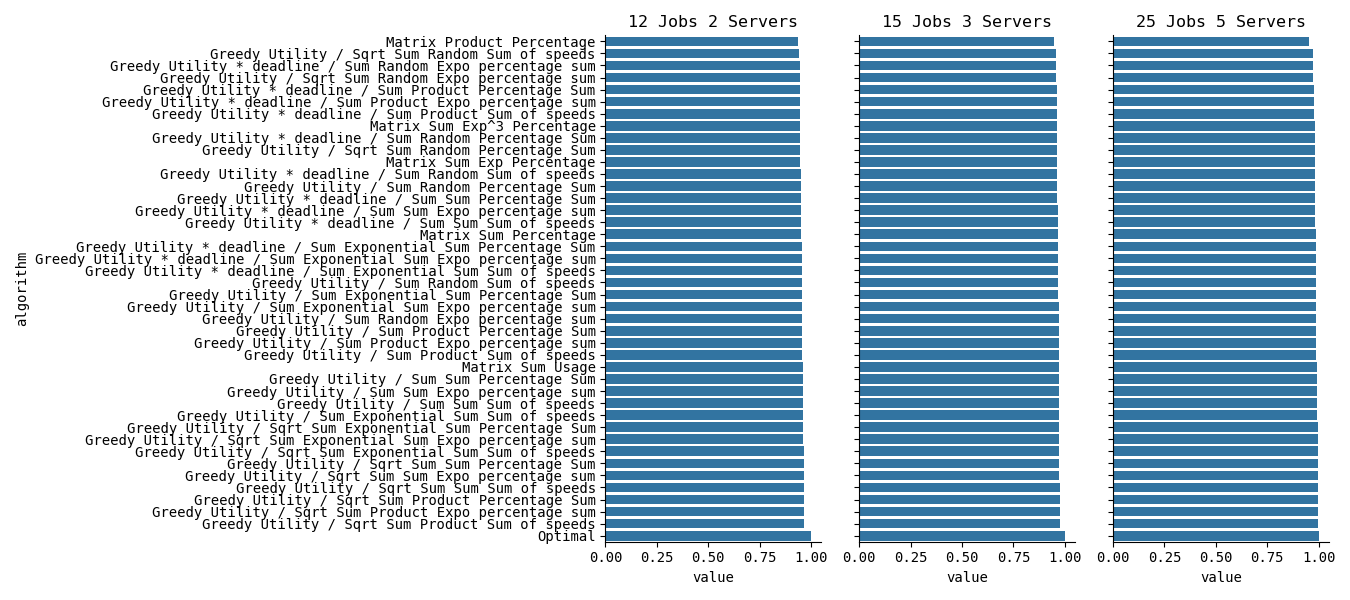
\includegraphics[width=1\linewidth, height=5cm]{./images/optimal_greedy_results.png}
    \caption{Greedy Results}
\end{figure}
\begin{figure}[H]
    \centering
    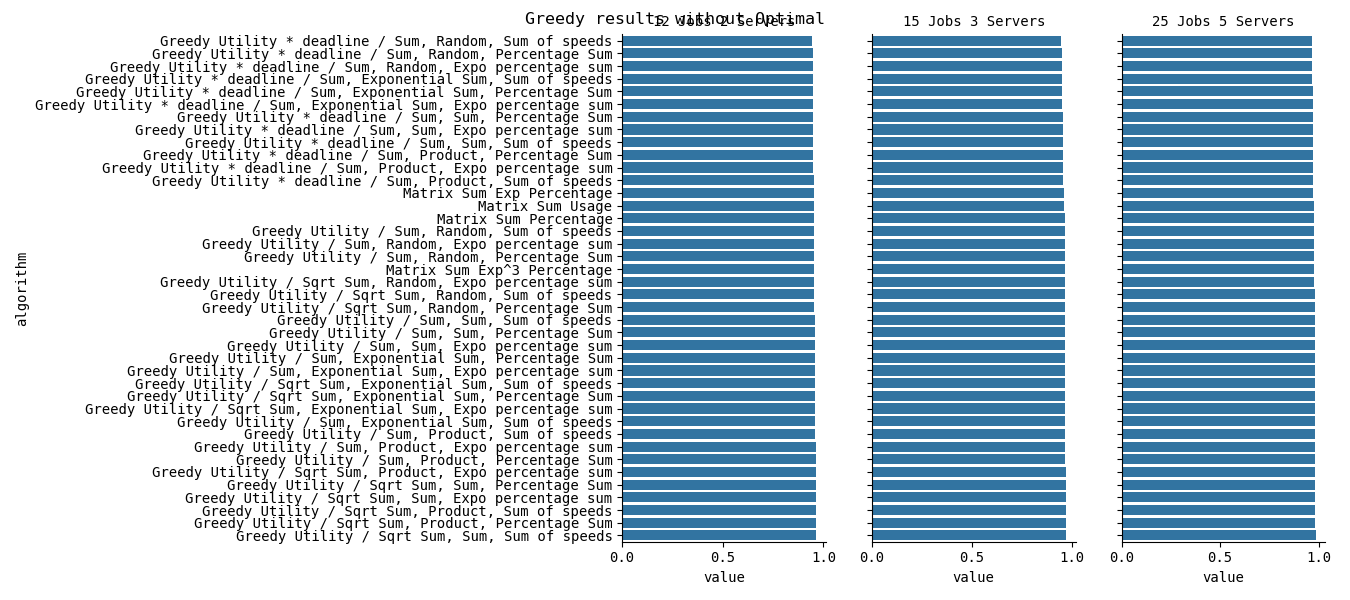
\includegraphics[width=1\linewidth, height=5cm]{./images/no_optimal_greedy_results.png}
    \caption{Greedy Results with the optimal algorithms}
\end{figure}

\section{Auctions}\label{sec:auction-idea}
While the greedy algorithm allows us to find near optimals for problems where we have perfect information about the
problem case like the job utility, this may be private information that the job owner doesnt want to reveal also
server would want to get paid for that work that they do. \\
We propose a iterative auctions where the job owner doesnt have to reveal it's true utility. In normal VCG auctions,
then the auctioneer will solve the problem to maximise the social welfare (total utility of allocated jobs) and
must find the optimal solution. Then for each job and server, the job or server is removed from the problem case and the
optimal is solved for that as well with the server's revenue it is paid and the job's cost being the social welfare of
the optimal solution minus the social welfare of the optimal without the job or server. This is extremely slow and
unscalable because of this so is not used often however has the properties that it is individually rational, truthful
bidding and incentive compatible. \\
Our iterative auctions uses the idea of VCG so that when a job asks to run on a server then the server will calculate
current revenue of the jobs running minus the revenue if the new job must be running on the server plus a price increase
factor. This is then the price for the job to run on the server as the new allocation with the job would be to a greater
revenue for the server than is currently allocated.

\subsection{Iterative Auction algorithm}\label{subsec:iterative-auctions-algorithm}
\begin{lstlisting}[language=Python]
unallocated_jobs = jobs
while len(unallocated_jobs):
    # Select a job, can be at random
    job = unallocated_jobs[0]

    # Calculate the minimum job price on all of the servers
    job_price, allocation_info = min((evaluate_job_price(job, server, epsilon=epsilon)
                                     for server in servers), key=lambda bid: bid[0])
        # Check if the job can pay the minimum price
        if job_price <= job.utility:
            # Uses the allocation info to create the new allocation on the selected server
            allocate_job(job_price, job, allocation_info, unallocated_jobs)
        else:
            # Remove job as the job can be run ever at a price lower than the job's true utility
            unallocated_jobs.remove(job)
\end{lstlisting}

\section{Iterative Auction Results}\label{sec:auctions-results}
\begin{figure}[H]
    \centering
    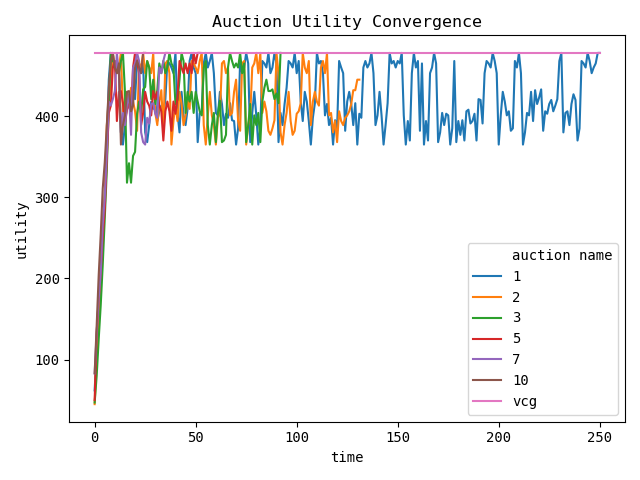
\includegraphics[width=1\linewidth]{../results/auction_utility_convergence.png}
    \caption{Auction Utility Convergence}
\end{figure}

%% TODO iterative auctions price difference to vcg


\end{document}
